\section{Amyotrofisk lateral sklerose}
ALS er en neurodegenerativ sygdom, der påvirker motorneuronerne i hjernen og rygsøjlen i takt med sygdommens fremskriden, hvilket resulterer i muskelsvaghed. En illustration af, hvordan ALS påvirker motorneuroner, ses af \autoref{fig:affectedneuron}. De første symptomer herpå er kramper, svaghed samt stive muskler, hvilket kan opstå som muskelsvaghed i arme eller ben, talebesvær eller svaghed i de muskler, som styrer respirationen. Symptomer, der begynder i arme eller ben kaldes 'limb onset ALS', mens talebesvær samt synkebesvær refereres til 'bulbar onset ALS'. 
Symptomerne og følgerne af ALS varierer fra patient til patient, hvorved nogle patienter først oplever muskelsvaghed i deres ben, mens andre oplever muskelsvaghed i deres hænder og arme eller besvær i form af tale- eller synkebesvær. \citep{miller2005} \citep{nationalinstitute2016}

 \begin{figure}[H]
\centering
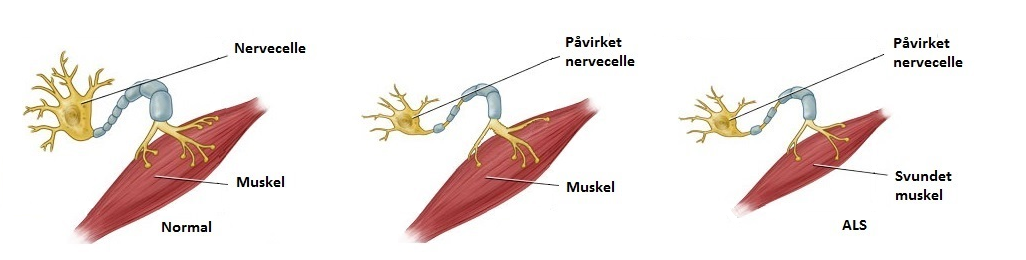
\includegraphics[width=0.5\textwidth]{figures/affectedneuron}
\caption{På figuren ses en upåvirket samt en degenereret motorneuron. Heraf ses det ligeledes, hvilken påvirkning ALS har på muskeler, hvortil det ses, at den degereret motorneurons muskel er svundet ind. \citep{drake2015}}
\label{fig:affectedneuron}
\end{figure}
 
Muskelsvagheden skyldes abnormiteter i de nedre motorneuroner. De nedre motorneuroner er de nerveceller, der videregiver information fra rygmarven til musklerne. Symptomer på abnormiteter i de nedre motorneuroner ses som muskelsvaghed samt muskelkramper og atrofi.
Ligeledes kan de øvre motorneuroner påvirkes. Disse motorneuroner sørger for kommunikationen mellem hjernen og de nedre motorneuroner i rygmarven. Dette medfører, at beskeden fra hjernen har komplikationer med at komme til det givne sted. Dette ses som spasticitet samt overdrevne reflekser.\citep{nationalinstitute2016} Opdelingen af de nedre samt øvre motorneuroner ses af \autoref{fig:motorneuroner}.
Årsagen til, at ALS opstår er oftest ukendt, dog ses en arvelighed i 5-10 \% af tilfældene. Herudaf anslås 20 \% til at have det muterede Superocide dismutase 1-gen (SOD-1), hvilket resulterer i tab af motorneuroner. \citep{miller2005}

\begin{figure}[H]
\centering
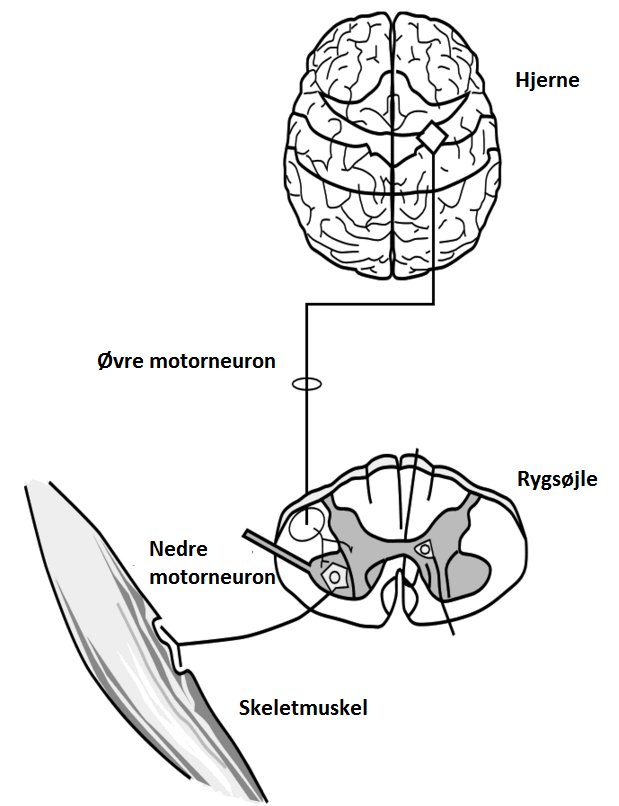
\includegraphics[width=0.5\textwidth]{figures/motorneuroner.png}
\caption{Figuren illustrerer opdelingen af de nedre samt øvre motorneuroner. \citep{miller2005}}
\label{fig:motorneuroner}
\end{figure}

På trods af, at ALS opleves individuelt både i forhold til sygdomsprogressionen samt, hvilke komplikationer de oplever, kan sygdommen inddeles i 3 stadier: et tidligt, midter og endeligt stadie. 
I det tidlige stadie kan patienter ignorere symptomerne, da disse fremstår som milde og kun påvirker mindre dele af kroppen. 
Ved det midterste stadie vil symptomerne begynde at udbrede sig, hvortil nogle muskler paralyseres. Andre muskler vil blive svagere med tiden, hvilket blandt andet kan medføre problemer med synkning og vejrtrækningen. I det endelige stadie vil de fleste voluntære muskler være paralyserede, og det vil derfor forringe deres mulighed for indtage føde eller væske normalt. Herudover vil patienter oftest i dette stadie miste even til selv at trække vejret, og bliver derfor afhængig af ventilationsstøtte. \citep{themusculardystrophyassociation2016} 
Den mest almindelige dødsårsag er respirationssvigt, hvilket oftest sker inden for 3 år efter diagnosen er stillet. 25 \% af patienterne har en overlevelsesrate på 5 år, og kun 10 \% lever længere end 10 år efter diagnosen er stillet. \citep{grehl2011} \citep{miller2005}




%Til at starte med kan mindre symptomer som besvær ved at gå op ad trapper opstå. Ligeledes kan patienterne være påvirket af dropfod, når de går. Herefter vil musklerne gradvist blive svagere, og med tiden vil patienterne ikke længere være i stand til at gå.\citep{tidy2015} 